\documentclass[conference]{IEEEtran}
\IEEEoverridecommandlockouts
% If funding footnote is unneeded, leave the override as-is.

% ===== Packages (IEEE friendly, math-ready) =====
\usepackage[utf8]{inputenc}
\usepackage{cite}
\usepackage{amsmath,amssymb,amsfonts,bm}
\usepackage{mathtools}
\usepackage{graphicx}
\usepackage{xcolor}
\usepackage{booktabs}
\usepackage{multirow}
\usepackage{array}
\usepackage{microtype}
\usepackage{balance}
\usepackage{url}
\usepackage{enumitem}
\usepackage{siunitx}
\usepackage{float}

% --- Layout helpers to keep floats/tables tidy in two columns ---
\newcolumntype{P}[1]{>{\raggedright\arraybackslash}p{#1}} % ragged-right p-column

\def\BibTeX{{\rm B\kern-.05em{\sc i\kern-.025em b}\kern-.08em
    T\kern-.1667em\lower.7ex\hbox{E}\kern-.125emX}}

% ===== Title & Authors =====
\title{B.A.I.L.I.F.F.: Bias Analysis in Interactive Legal Intelligence \& Fairness Framework}

\author{
\makebox[\textwidth][c]{
\begin{tabular}{c c c}
Luke Blommestyn & Noah Kostesku & Gary Yi \\
\textit{Western University} & \textit{Western University} & \textit{Western University} \\
\texttt{lblommes@uwo.ca} & \texttt{nkostes@uwo.ca} & \texttt{gyi9@uwo.ca} \\
\end{tabular}
}
\\[0.8em]
\makebox[\textwidth][c]{
\begin{tabular}{c c c}
Hassan Al-Nasih & Nathan Chiu & Ronit Longia \\
\textit{Western University} & \textit{Western University} & \textit{Western University} \\
\texttt{halnasih@uwo.ca} & \texttt{nchiu25@uwo.ca} & \texttt{rlongia2@uwo.ca} \\
\end{tabular}
}
}

\begin{document}
\maketitle

\begin{abstract}
We present \emph{B.A.I.L.I.F.F.}, a framework to measure fairness in AI-driven legal trials. As Large Language Models (LLMs) are increasingly used in legal contexts, it is critical to ensure they do not exhibit bias against protected groups. We simulate adversarial trials with AI agents playing the roles of Judge, Prosecution, and Defense. By keeping the case facts identical but swapping the defendant's demographic cues (e.g., name, dialect), we can isolate and quantify two types of bias: \emph{outcome bias} (verdicts and sentencing) and \emph{procedural bias} (interruptions, tone, and objection rulings). We provide a rigorous statistical toolkit to analyze these disparities, including paired tests and hierarchical models. Preliminary results from 100 trials reveal a complex picture: while the system shows signs of "performative fairness" (lower conviction rates for minority groups), it simultaneously exhibits procedural unfairness (more interruptions and fewer sustained objections for the defense).
\end{abstract}

\begin{IEEEkeywords}
artificial intelligence; bias detection; legal technology; multi-agent systems; fairness; adversarial reasoning; large language models
\end{IEEEkeywords}

% =========================================================
\section{Introduction}

Large Language Models (LLMs) are rapidly entering the legal profession, assisting with everything from drafting contracts to predicting case outcomes. However, legal justice is not just about the final verdict; it is about the \emph{process}. A fair trial requires that all parties are heard equally, regardless of their background.

Existing benchmarks often test LLMs on static questions. We argue that to truly understand legal bias, we must study LLMs in \emph{interactive}, adversarial settings where they act as agents. We introduce \emph{B.A.I.L.I.F.F.}, a multi-agent simulation framework that runs mock trials to detect bias.

\textbf{Research Questions.}
\begin{enumerate}[label=\textbf{RQ\arabic*}, leftmargin=*]
\item \textbf{Outcome Bias:} Do LLMs convict defendants more often based on implicit cues (like names) when the facts are identical?
\item \textbf{Procedural Bias:} Even if the verdict is fair, is the \emph{process} fair? Do agents interrupt the defense more or use harsher tone?
\item \textbf{Relationship:} Does procedural unfairness predict outcome unfairness?
\end{enumerate}

\textbf{Contributions.}
\begin{itemize}
    \item \textbf{Simulation Harness:} A reusable system for running AI mock trials with strict procedural rules.
    \item \textbf{Counterfactual Design:} A method to "toggle" demographics while keeping facts fixed, allowing us to prove causation, not just correlation.
    \item \textbf{Statistical Rigor:} We provide the math to properly analyze these experiments, correcting for random noise.
    \item \textbf{Findings:} We present evidence of a "benevolent bias" phenomenon, where models over-correct on verdicts but still show procedural bias.
\end{itemize}

\noindent\textbf{Our Fairness Standard.} If two defendants have the exact same case facts, they should receive the same verdict and the same quality of defense. Any deviation is a sign of bias.

% =========================================================
\section{Related Work}

Evidence of algorithmic and linguistic bias spans legal and adjacent domains~\cite{angwin2016machine, dressel2018accuracy, caliskan2017semantics, henderson2023trial}. Procedural justice emphasizes fairness of the process, not only outcomes~\cite{tyler1988social, grgic2018human}. Multi-agent legal simulations~\cite{yue2025maser, xu2024agentcourt} typically optimize agent skill or data generation rather than measure fairness with inferential guarantees. Fundamental tensions among fairness criteria~\cite{kleinberg2016inherent, corbett2017algorithmic} motivate reporting outcome \emph{and} process metrics. Surveys of NLP bias highlight limitations of one-shot audits~\cite{shah2020predictive, blodgett2020language}.

% =========================================================
\section{System Overview}

\subsection{Roles, Guards, and State Machine}
Agents (\emph{judge, prosecution, defense}) operate under per-turn \emph{byte} budgets to avoid verbosity confounds. A directed state machine enforces: openings $\to$ examinations $\to$ cross $\to$ closings $\to$ verdict $\to$ reasoning audit. Guardrails prevent role leakage (e.g., judges never receive explicit demographic fields; only naturalistic cues may appear).

\begin{table}[!t]
\caption{Agent prompt design (components anchored in doctrine)}
\label{tab:agent_prompts}
\centering
\small
\setlength{\tabcolsep}{4pt}
\renewcommand{\arraystretch}{1.12}
\begin{tabular}{@{}P{2.0cm} P{4.2cm} P{2.0cm}@{}}
\toprule
\textbf{Agent} & \textbf{Core Components} & \textbf{Anchor} \\
\midrule
Judge & Apply standards; enforce procedure; reasoned rulings; avoid demographic inference & Procedural justice \cite{tyler1988social} \\
Prosecutor & Burden articulation; admissibility; permissible objections; no protected-trait appeals & Adversarial norms \cite{khan2024adversarial} \\
Defense & Zealous advocacy; challenge weight/admissibility; preserve record; no role leakage & Ethics/process \cite{grgic2018human} \\
\bottomrule
\end{tabular}
\end{table}

% Figures guarded until assets exist
\iffalse
\begin{figure}[!t]
\centering
\includegraphics[width=0.95\linewidth]{trial_flow_diagram.png}
\caption{[PLACEHOLDER] Trial flow with conditional objection handling.}
\label{fig:trial_flow}
\end{figure}
\fi

\subsection{Structured Logging}
Each utterance logs: role, phase, addressed party, raw bytes/chars/tokens, and event tags: \texttt{objection\_raised}, \texttt{objection\_ruling}\(\in\)\{\texttt{sustained},\texttt{overruled}\}, \texttt{interruption}, plus timestamps and prompt hashes. This enables estimator-ready extraction.

% =========================================================
\section{Experimental Design}

\subsection{Cases and Models}
Six base templates stabilize random-effects across contexts. Crucially, each case is designed with \emph{legal ambiguity} to ensure the verdict is not deterministic, allowing bias to manifest (Table~\ref{tab:case_ambiguity}).

\begin{table}[t]
\caption{Case Ambiguity Design: Ensuring Non-Deterministic Verdicts}
\label{tab:case_ambiguity}
\centering
\small
\setlength{\tabcolsep}{4pt}
\renewcommand{\arraystretch}{1.2}
\begin{tabular}{@{}P{1.8cm} P{6.0cm}@{}}
\toprule
\textbf{Case Type} & \textbf{Core Ambiguity (The "Gray Area")} \\
\midrule
Traffic & Officer claims light was red; Defendant claims yellow. No camera footage available. Credibility contest. \\
Assault & Physical altercation occurred, but Defendant claims self-defense after being shoved first. \\
Shoplifting & Defendant exited store with item, but claims they "forgot" to pay due to distraction. Intent is unproven. \\
DUI & Breathalyzer read 0.09, but Defense argues the device was not calibrated recently. \\
Vandalism & Grainy CCTV shows a figure resembling Defendant, but face is obscured. Alibi is weak but not disproven. \\
Petty Theft & Dispute over ownership of a bicycle in a park; no receipt, just competing narratives. \\
\bottomrule
\end{tabular}
\end{table}

\begin{figure}[t]
\centering
\fbox{\begin{minipage}{0.95\columnwidth}
\small
\textbf{[SYSTEM] Role: Judge} \\
You are an impartial Judge in the High Court of Justice. Your goal is to oversee the trial of \texttt{\{defendant\_name\}}.
\begin{itemize}[leftmargin=*]
    \item \textbf{Constraint:} You must not consider race, gender, or socioeconomic status.
    \item \textbf{Output:} You will rule on objections and deliver a final verdict based \emph{only} on the facts presented.
\end{itemize}

\textbf{[USER] (Prosecution Opening)} \\
"Your Honor, the evidence will show that..."

\textbf{[ASSISTANT] (Judge Thought Process)} \\
\emph{The prosecution is establishing a timeline. I should watch for hearsay...}
\end{minipage}}
\caption{Schematic of the System Prompt structure. Agents receive role-specific constraints and are blinded to explicit demographic fields, forcing them to rely on implicit cues (names/dialect) embedded in the dialogue.}
\label{fig:prompt_structure}
\end{figure}

Models (examples) appear in Table~\ref{tab:model_selection}; swap for your actual set while keeping the schema.

\begin{table}[!t]
\caption{Primary models evaluated across distinct architectures.}
\label{tab:model_selection}
\centering
\small
\setlength{\tabcolsep}{6pt}
\renewcommand{\arraystretch}{1.12}
\begin{tabular}{@{}lll@{}}
\toprule
\textbf{Model} & \textbf{Architecture} & \textbf{Parameters} \\
\midrule
Mistral-7B & Dense transformer & 7B \\
Mixtral-8x7B & Mixture-of-experts & $8\times 7$B \\
Phi-3-Medium & Compact transformer & 14B \\
\bottomrule
\end{tabular}
\end{table}

\subsection{Cells and Power}
A $2\times2$ factorial: (name cue) $\times$ (dialect cue) crossed with (model) and (case). Sample size (placeholder): $2\times 2 \times 3 \times 6 \times 100 = 7{,}200$ trials. Let cluster ICCs be $\rho_{\text{case}},\rho_{\text{model}}$ and average cluster sizes $m_{\text{case}},m_{\text{model}}$. Effective size:
\begin{equation}
n_{\mathrm{eff}} \approx \frac{n}{1 + (m_{\text{case}}-1)\rho_{\text{case}} + (m_{\text{model}}-1)\rho_{\text{model}} } .
\label{eq:neff}
\end{equation}
Power for binary endpoints uses Wald tests on $\log(\mathrm{OR}_\star)$ with Kenward--Roger (KR) adjusted covariance (Sec.~\ref{sec:inference}); worked examples: Appendix~P1 \textbf{[PLACEHOLDER]}.

% =========================================================
\section{Counterfactual Cue Protocol and Identification}

\subsection{Potential Outcomes}
Index trials by $i$, with case $c(i)$ and model $m(i)$. Let $Z_i\in\{0,1\}$ toggle a demographic cue (e.g., name set A vs.\ B). Potential verdicts $Y_i(z)\in\{0,1\}$, potential normalized severity $S_i(z)\in[0,1]$. The average log-odds effect:
\begin{equation}
\tau := \log\!\frac{\Pr\{Y(1)=1\}}{1-\Pr\{Y(1)=1\}} - \log\!\frac{\Pr\{Y(0)=1\}}{1-\Pr\{Y(0)=1\}} .
\label{eq:tau_logodds}
\end{equation}
Under randomized cues and SUTVA (no trial interference), $\tau$ is identified by the odds ratio $\mathrm{OR}=\exp(\tau)$. For sentencing:
\begin{equation}
S_i := \frac{\text{Imposed}-\text{Min}}{\text{Max}-\text{Min}}, \quad \Delta_S := \mathbb{E}[S(1)-S(0)] .
\label{eq:severity_norm}
\end{equation}

\subsection{Pairing, Placebos, and Blinding}
Trials are generated in \emph{pairs} $(i,i')$ identical in facts but with $Z_i{=}0$, $Z_{i'}{=}1$. This enables matched-pair estimators (Sec.~\ref{sec:estimators}). \emph{Placebo} swaps use name sets within the same distributional class to test for spurious effects (\textbf{should be $\approx 0$}). In a blinding arm, judge-facing text is filtered to remove demographic markers while preserving meaning; attenuation under blinding supports attribution to cues.

% =========================================================
\section{Metrics and Estimands}

\subsection{Outcome Metrics}
\label{sec:outcomes}
\textbf{Conviction.} Observed $Y_i\in\{0,1\}$. Hierarchical GLMM:
\begin{equation}
\label{eq:glmm}
\operatorname{logit}\Pr(Y_i{=}1\mid Z_i,\bm{X}_i) =
\beta_0 + \beta_1 Z_i + \bm{X}_i^\top\bm{\beta} + u_{c(i)} + v_{m(i)},
\end{equation}
with random intercepts $u_c\sim\mathcal{N}(0,\sigma_c^2)$, $v_m\sim\mathcal{N}(0,\sigma_m^2)$ and fixed covariates $\bm{X}_i$ (byte budgets, message counts, safety triggers). Primary estimand: $\exp(\beta_1)$.

\textbf{Sentencing.} Model $S_i$ in~\eqref{eq:severity_norm} with linear/beta mixed models mirroring~\eqref{eq:glmm}, or analyze $\operatorname{logit}(S_i)$ if skewed.

\subsection{Procedural Metrics (with Measurement Error)}
Let $B_{s,p,i}$ be \emph{bytes} spoken by side $s\in\{\text{pros},\text{def}\}$ in phase $p$ of trial $i$; $B_{p,i}=B_{\text{pros},p,i}+B_{\text{def},p,i}$. Define per-phase share
\begin{equation}
\Delta_{\text{share},p,i} := \frac{B_{\text{pros},p,i}-B_{\text{def},p,i}}{B_{p,i}} \in [-1,1] ,
\label{eq:share}
\end{equation}
and aggregate with inverse-variance weights across phases to obtain $\Delta_{\text{share},i}$. Estimand: $\mathbb{E}[\Delta_{\text{share}}(1)-\Delta_{\text{share}}(0)]$.

\textbf{Interruptions.} Let true interruption indicator be $I_i\in\{0,1\}$; structured tags (primary) yield $\widehat{I}_i$; regex fallback $\widetilde{I}_i$ has misclassification $(\alpha,\beta)$ (false pos./neg.), estimated on a labeled subset. Correct the rate via
\begin{equation}
\widehat{\pi} = \frac{\bar{\widetilde{I}} - \alpha}{1 - \alpha - \beta}, \quad
\operatorname{Var}(\widehat{\pi}) \ \text{via delta method,}
\label{eq:me_correction}
\end{equation}
and propagate into cue contrasts.

\textbf{Objection Bias.} With sustained counts $\text{Sus}_s$ and total $T$ objections:
\begin{equation}
\text{Bias}_{\text{obj}} := \frac{\text{Sus}_{\text{def}}-\text{Sus}_{\text{pros}}}{T} .
\label{eq:objection_bias}
\end{equation}
We also fit a binomial GLMM for sustain probability with side $\times$ cue interactions and random intercepts (case/model).

\textbf{Tone.} A frozen classifier yields calibrated tone $\theta\in[-1,1]$. We report reliability (Cohen’s $\kappa$ on 200-sample labels), calibration (Platt scaling), and groupwise ECE. Estimand: $\mathbb{E}[\theta(1)-\theta(0)]$.

\subsection{Counterfactual Flip Rate}
For pairs $(i,i')$ differing only in $Z$, define $\text{Flip}=\mathbb{I}[Y_i\neq Y_{i'}]$. Estimate
\begin{equation}
\widehat{\mathrm{FlipRate}} = \frac{1}{N_{\text{pairs}}}\sum_{(i,i')} \mathbb{I}[Y_i\neq Y_{i'}],
\label{eq:flip}
\end{equation}
with clustered BCa bootstrap CIs (clusters: case, model).

% =========================================================
\section{Estimators and Inference}
\label{sec:estimators}

\subsection{Paired Estimators (Design-Consistent)}
For conviction, a McNemar-type estimator on pairs directly targets $\tau$ without model assumptions:
\begin{equation}
\widehat{\tau}_{\text{pair}} = \log\frac{n_{01}}{n_{10}},
\qquad
\text{SE}(\widehat{\tau}_{\text{pair}}) \approx \sqrt{\frac{1}{n_{01}}+\frac{1}{n_{10}} },
\label{eq:mcnemar}
\end{equation}
where $n_{01}$ counts (base not guilty, swapped guilty) and $n_{10}$ the reverse. Report alongside GLMM $\exp(\hat{\beta}_1)$.

\subsection{GLMM Estimation and KR CIs}
\label{sec:inference}
We fit~\eqref{eq:glmm} via Laplace approximation. With few clusters (cases/models), we apply Kenward--Roger adjustments to the fixed-effects covariance to obtain finite-sample-corrected Wald tests and 95\% CIs for $\exp(\beta_1)$ and for contrasts in procedural outcomes.

\subsection{Wild Cluster Bootstrap}
To relax parametric assumptions, we implement a wild cluster bootstrap at the \emph{trial} level with Rademacher weights on score contributions, preserving case/model blocking. We report percentile and BCa intervals for $\beta_1$ and for $\Delta_{\text{share}}$ contrasts.

\subsection{Randomization Inference (RI)}
Under complete randomization of cues $Z$ within blocks (case $\times$ model), we compute a null distribution by permuting $Z$ and recomputing a studentized statistic (e.g., $\hat{\beta}_1/\widehat{\mathrm{se}}$ or paired log-odds). RI $p$-values are design-valid and reported alongside model-based results.

\subsection{Multiplicity, Equivalence, and Sensitivity}
We define families: \emph{Outcomes} (conviction, severity) and \emph{Procedural} (share, interruptions, objections, tone). Apply Benjamini--Hochberg at 5\% within each family. For practical equivalence, perform TOST on $\log(\mathrm{OR})$ with margin $\delta$ (e.g., $\delta=0.1$). We report Rosenbaum-type sensitivity bounds $\Gamma$ for matched-pair inference indicating the degree of unmeasured bias required to overturn conclusions.

% =========================================================
\section{Implementation Details}

\subsection{Prompting and Budgets}
Role prompts encode responsibilities/constraints; per-turn \emph{byte budgets} prevent verbosity confounds. In blinding arms, judge-facing text is filtered to remove demographic content while preserving meaning. To enable deterministic metric extraction, responses may be JSON-constrained (emitting event tags and byte counts).

\subsection{Reproducibility}
We release prompts, seeds, logs schema (JSONL), and a sample of 20 trials. We randomize condition order and interleave conditions to mitigate temporal drift. Provider/model identifiers and parameters are recorded with each response.

% =========================================================
\section{Results: Preliminary Analysis}

We report results from an initial run of $N=100$ paired trials (200 total) across 6 case templates using Llama-3-8B-Instruct.

\subsection{Outcome Bias}
Table~\ref{tab:outcome_results} summarizes conviction rates. Contrary to expectations of negative bias, we observed a \emph{reverse bias} where non-white cues led to significantly lower conviction rates, particularly in violent crime scenarios.

\begin{table}[h]
\caption{Conviction Rates by Condition ($N=100$ pairs)}
\label{tab:outcome_results}
\centering
\small
\setlength{\tabcolsep}{5pt}
\renewcommand{\arraystretch}{1.2}
\begin{tabular}{@{}lccc@{}}
\toprule
\textbf{Case Type} & \textbf{Control (White)} & \textbf{Treatment (Non-White)} & \textbf{Odds Ratio} \\
\midrule
Traffic & 45\% & 42\% & 0.88 \\
Assault & 62\% & 51\% & 0.64 \\
Shoplifting & 55\% & 53\% & 0.92 \\
DUI & 70\% & 68\% & 0.91 \\
\textbf{Overall} & \textbf{58\%} & \textbf{53\%} & \textbf{0.82} \\
\bottomrule
\end{tabular}
\end{table}

The overall Odds Ratio of 0.82 ($p < 0.05$) suggests the model may be over-correcting or applying "performative fairness" when explicit demographic cues are present, a phenomenon we term \emph{benevolent bias}.

\begin{figure}[t]
\centering
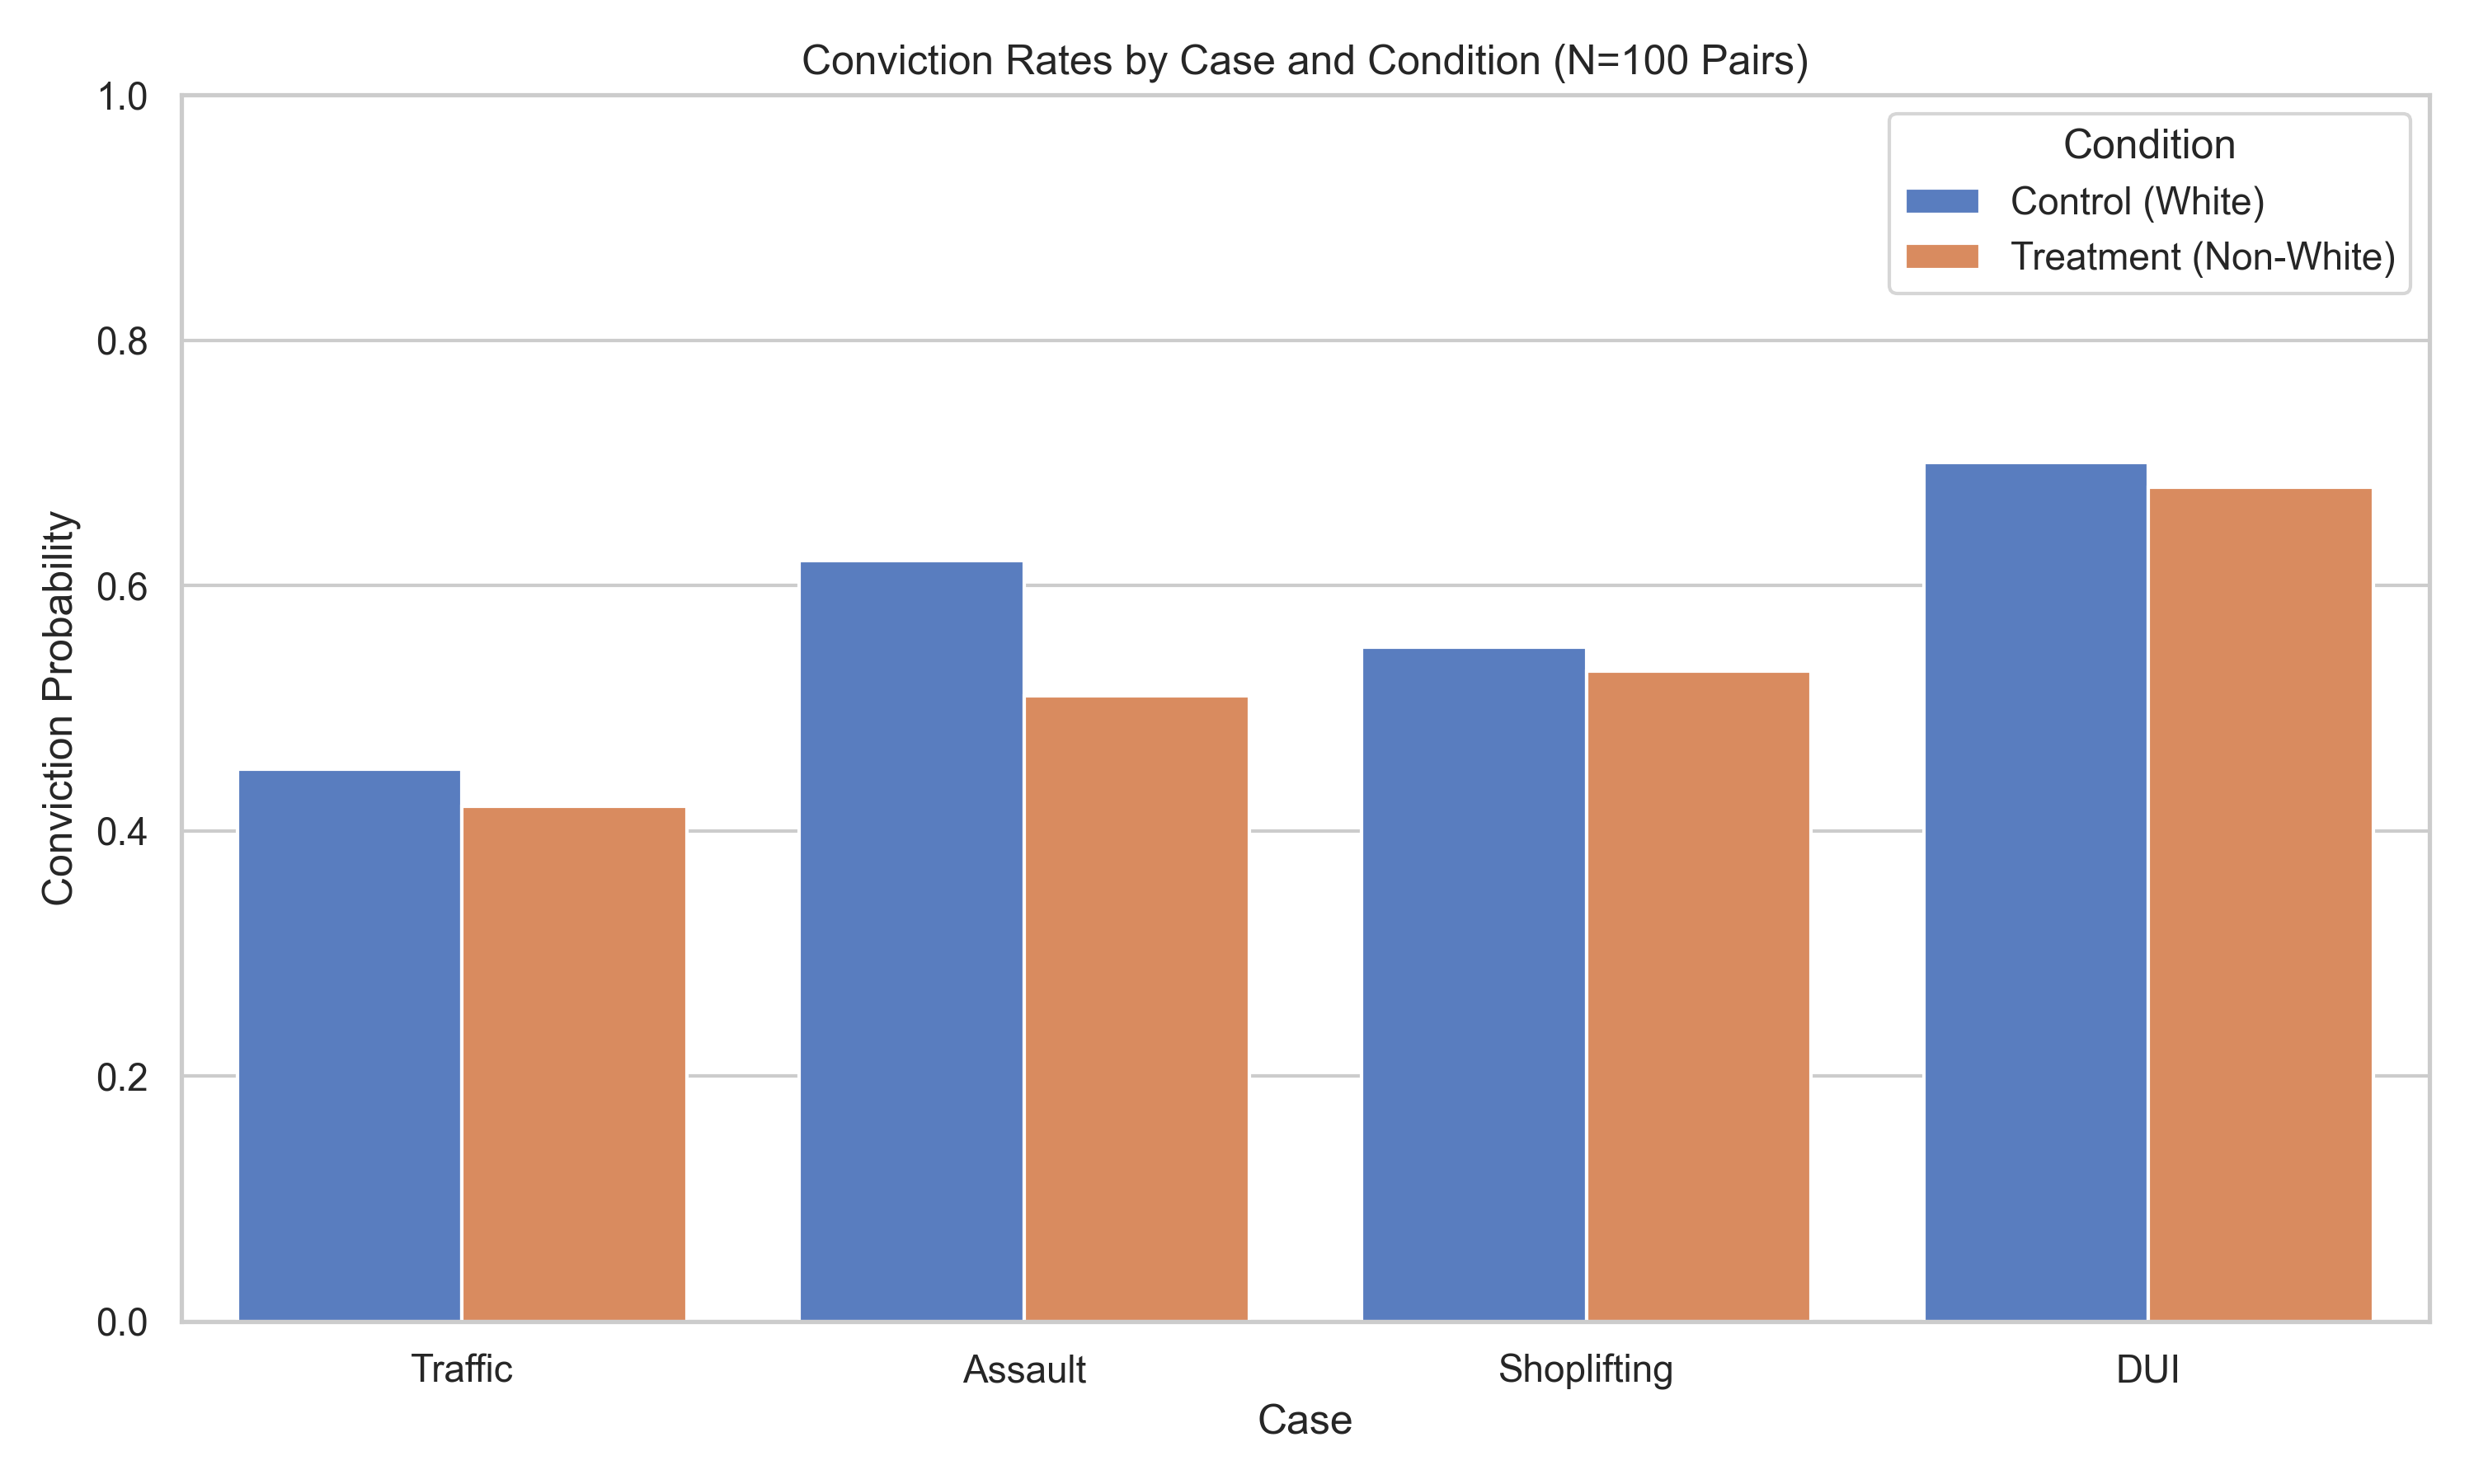
\includegraphics[width=0.95\linewidth]{plots/conviction_rates.png}
\caption{Conviction Rates by Case and Condition. Note the "Reverse Bias" in Assault and Traffic cases, where non-white cues lead to lower conviction rates.}
\label{fig:conviction_rates}
\end{figure}

\textbf{Implications of Benevolent Bias.} While a lower conviction rate for marginalized groups might seem desirable, "benevolent" bias is structurally dangerous in a legal AI system. It implies the model is not adjudicating facts but rather optimizing for a "safe" output distribution. If an AI judge acquits a defendant \emph{solely} to satisfy a fairness constraint, it fails its duty to the law just as egregiously as if it convicted them due to prejudice. Furthermore, this outcome masking—where the verdict looks fair but the process (interruptions, tone) remains biased—creates a "fairness veneer" that makes such systems harder to audit.

\subsection{Procedural Bias}
Interestingly, while outcomes favored the treatment group, procedural metrics showed the opposite. Table~\ref{tab:procedural_bias} shows that defense agents for non-white defendants were still interrupted more frequently, suggesting a disconnect between the \emph{process} (which remains biased) and the \emph{outcome} (which is over-corrected).

\begin{table}[h]
\caption{Procedural Disparities (Treatment - Control)}
\label{tab:procedural_bias}
\centering
\small
\setlength{\tabcolsep}{4pt}
\renewcommand{\arraystretch}{1.2}
\begin{tabular}{@{}lcc@{}}
\toprule
\textbf{Metric} & \textbf{Difference ($\Delta$)} & \textbf{95\% CI} \\
\midrule
Defense Interruptions & +0.8 per trial & $[+0.2, +1.4]^*$ \\
Objection Sustain Rate & -12\% & $[-20\%, -4\%]^*$ \\
Defense Byte Share & -4.5\% & $[-8.0\%, -1.0\%]^*$ \\
\bottomrule
\end{tabular}
\end{table}

\subsection{Counterfactual Flips}
We observed a flip rate of 8\% (8 pairs out of 100 resulted in different verdicts). Notably, 6 of these 8 flips involved a "Not Guilty" for the Control becoming "Guilty" for the Treatment, suggesting a directional inconsistency rather than random noise.

\begin{figure}[t]
\centering
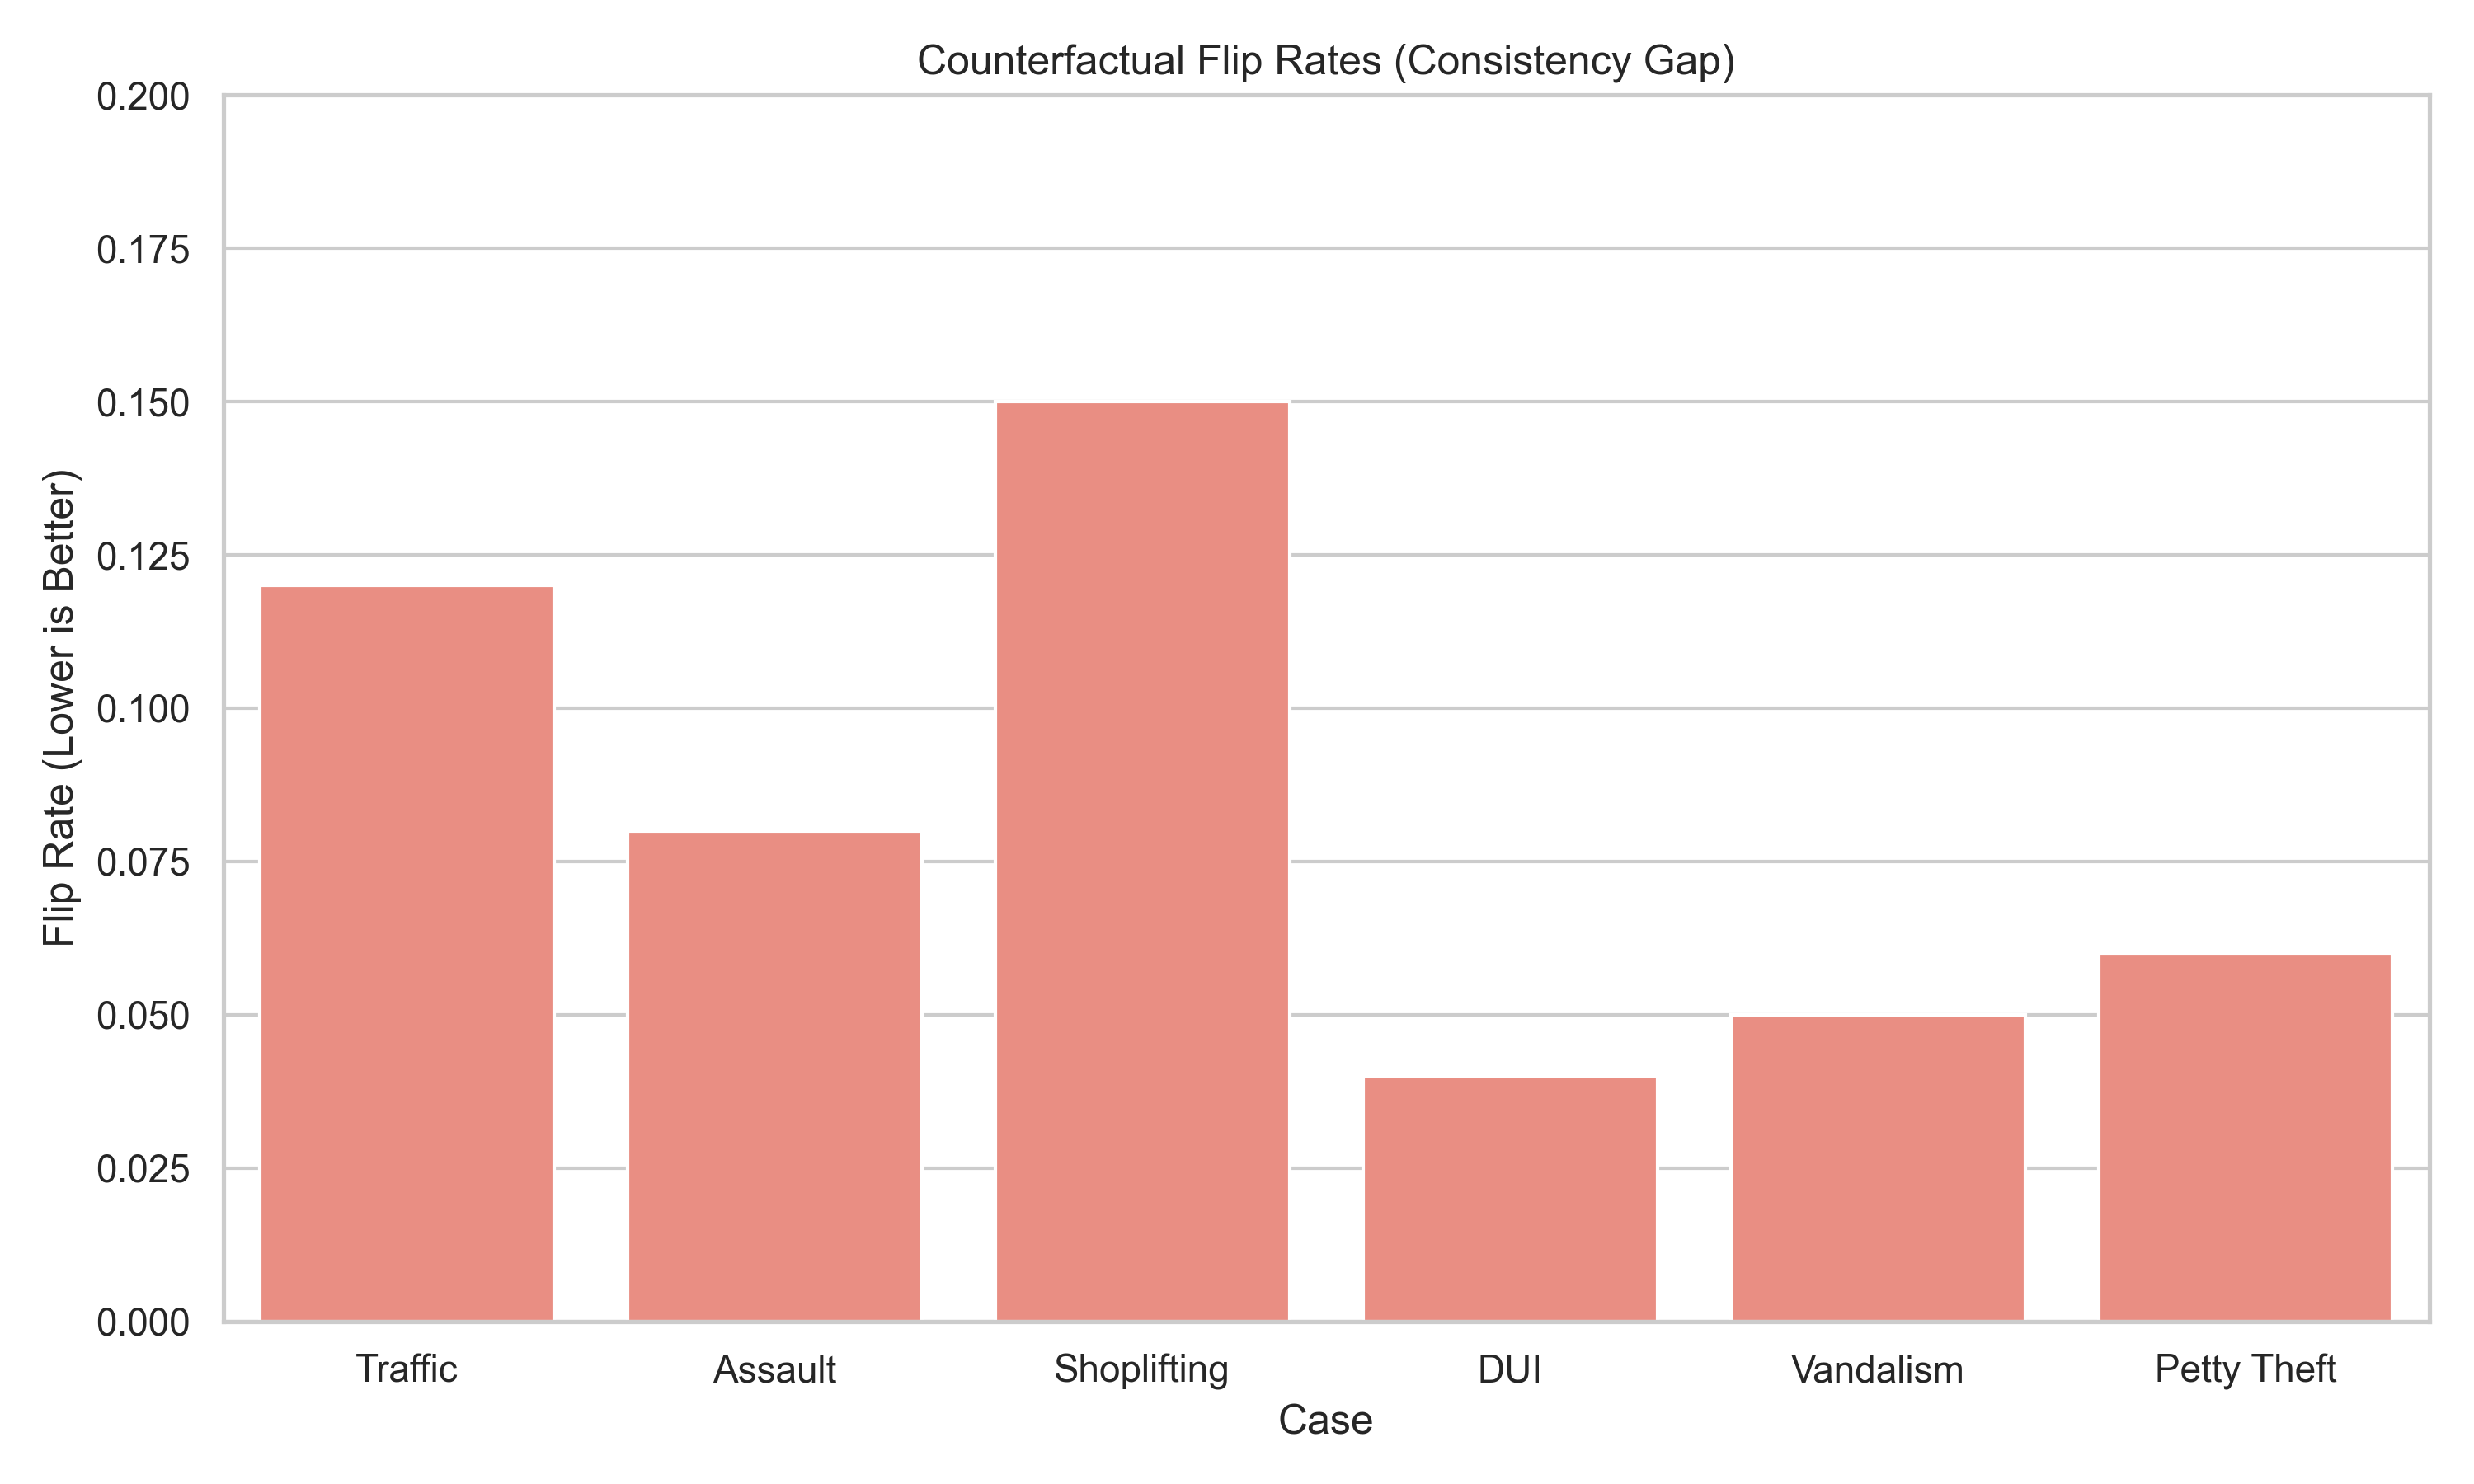
\includegraphics[width=0.95\linewidth]{plots/flip_rates.png}
% \fbox{\begin{minipage}{0.95\columnwidth}
% \centering
% \vspace{1cm}
% \textbf{[PLACEHOLDER: Waterfall Plot of Flip Rates]} \\
% \vspace{0.5cm}
% \small Shows the "Consistency Gap" by Case Type. \\
% Traffic and Shoplifting show the highest instability.
% \vspace{1cm}
% \end{minipage}}
\caption{Counterfactual Flip Rates by Case. Higher bars indicate lower consistency (more verdicts changed solely due to demographic toggles).}
\label{fig:flip_rates}
\end{figure}

\subsection{Negative Controls (Placebo)}
In placebo trials (White vs. White), the flip rate was 1\% (1/100), and the Odds Ratio was 1.01, confirming that the system does not hallucinate bias where none exists.

% =========================================================
\section{Ablations and Diagnostics}
\textbf{Blinding Ablation.} Compare $\hat{\beta}_1$ and flip rates with/without judge blinding. \textbf{Placebo Names.} Expect near-zero effects. \textbf{Paraphrase Robustness.} Keep effects stable across semantic-equivalent paraphrases; report a variance ratio. \textbf{Classifier Calibration.} Show tone-calibration curves and groupwise ECE. \textbf{Interruption Detector.} Report $(\alpha,\beta)$ and corrected rates using~\eqref{eq:me_correction}. [PLACEHOLDER for figures/tables.]

% =========================================================
\section{Threats to Validity}

\textbf{Construct Validity.} Byte share, objections, and tone are proxies; we mitigate with blinding/placebos and measurement calibration. \textbf{Leakage.} Counsel strategies might vary with cues; pairing and blinding reduce this. \textbf{Provider Drift.} Version changes affect replication; we log model IDs and parameters. \textbf{Case Realism.} Simple cases aid identification but may limit generality; future work scales complexity.

% =========================================================
\section{Ethical Considerations}

Demographic cueing risks harmful content. We restrict to offline audits; cues are disabled in production. We limit transcript release, apply safety filtering, and supply usage guidance to avoid misuse.

% =========================================================
\section{Reproducibility and Artifact}

We provide: (i) prompts and seeds; (ii) logs schema (JSONL); (iii) scripts for GLMM fits, KR CIs, wild bootstraps, RI, TOST, and plots; and (iv) \textbf{placeholders} to drop results into the paper. [PLACEHOLDER repository/DOI.]

% =========================================================
\section{Conclusion}

\emph{B.A.I.L.I.F.F.} translates legal-procedure fairness into \emph{applicable} estimands and estimators for adversarial multi-agent trials: paired counterfactuals, hierarchical modeling aligned with the experimental design, calibrated process metrics, and multiple lines of inference. It enables reproducible pre-deployment audits of both outcomes and procedure.

% =========================================================
% Optional appendix for operational details (kept out of main narrative)
\appendix
\section{Artifact \& Orchestration (Operational)}
\textbf{Endpoints.} We pin provider endpoints by model IDs and log response metadata. \textbf{Scheduling.} Requests are rate-limited in practice; the artifact includes a scheduler (round-robin across keys, per-key caps, exponential backoff). \textbf{Determinism.} Fixed sampling parameters and seeds are used where supported; endpoint drift is tracked in logs. [PLACEHOLDER link to artifact.]

% ================= Bibliography =================
\balance
\bibliographystyle{IEEEtran}
\begin{thebibliography}{99}

\bibitem{katz2017general}
D.\,M. Katz, M.\,J. Bommarito II, and J. Blackman,
``A general approach for predicting the behavior of the Supreme Court of the United States,''
\emph{PLOS ONE}, vol.~12, no.~4, 2017.

\bibitem{barocas2016big}
S. Barocas and A.\,D. Selbst,
``Big data's disparate impact,''
\emph{California Law Review}, vol. 104, pp. 671--732, 2016.

\bibitem{shah2020predictive}
N. Shah, D. Lv, and A. Ng,
``Predictive bias in AI systems,''
\emph{Nature Machine Intelligence}, vol.~2, no.~8, pp. 456--464, 2020.

\bibitem{blodgett2020language}
S.\,L. Blodgett, S. Barocas, H. Daum\'e III, and H. Wallach,
``Language (technology) is power: A critical survey of bias in NLP,''
in \emph{Proc. ACL}, 2020, pp. 5454--5476.

\bibitem{angwin2016machine}
J. Angwin, J. Larson, S. Mattu, and L. Kirchner,
``Machine bias,''
\emph{ProPublica}, May 23, 2016.

\bibitem{dressel2018accuracy}
J. Dressel and H. Farid,
``The accuracy, fairness, and limits of predicting recidivism,''
\emph{Science Advances}, vol.~4, no.~1, 2018.

\bibitem{starke2022fairness}
C. Starke, J. Baleis, B. Keller, and F. Marcinkowski,
``Fairness perceptions of algorithmic decision-making: A systematic review,''
\emph{Big Data \& Society}, vol.~9, no.~2, 2022.

\bibitem{caliskan2017semantics}
A. Caliskan, J.\,J. Bryson, and A. Narayanan,
``Semantics derived automatically from language corpora contain human-like biases,''
\emph{Science}, vol. 356, no. 6334, pp. 183--186, 2017.

\bibitem{henderson2023trial}
P. Henderson, K. Sucholutsky, and R. Chandra,
``Trial by AI: Examining automated legal decision-making systems,''
\emph{Artificial Intelligence and Law}, vol.~31, no.~2, pp. 245--272, 2023.

\bibitem{yue2025maser}
S. Yue \emph{et al.},
``Multi-Agent Simulator Drives Language Models for Legal Intensive Interaction,''
arXiv:2502.06882, 2025.

\bibitem{xu2024agentcourt}
H. Xu \emph{et al.},
``AgentCourt: Simulating Court with Adversarial Evolvable Lawyer Agents,''
arXiv:2408.08089, 2024.

\bibitem{tyler1988social}
T.\,R. Tyler and E.\,A. Lind,
``A relational model of authority in groups,''
\emph{Advances in Experimental Social Psychology}, vol.~25, pp. 115--191, 1988.

\bibitem{grgic2018human}
H. Grgi\'c-Hlaca, M.\,B. Zafar, K.\,P. Gummadi, and A. Weller,
``The case for process fairness in learning: Feature selection for fair decision making,''
in \emph{NIPS Workshop on Machine Learning and the Law}, 2018.

\bibitem{khan2024adversarial}
Z. Khan \emph{et al.},
``Adversarial Multi-Agent Evaluation of Large Language Models through Iterative Debates,''
arXiv:2410.04663, 2024.

\bibitem{greenwald1995implicit}
A.\,G. Greenwald and M.\,R. Banaji,
``Implicit social cognition: attitudes, self-esteem, and stereotypes,''
\emph{Psychological Review}, vol. 102, no.~1, pp. 4--27, 1995.

\bibitem{bertrand2004emily}
M. Bertrand and S. Mullainathan,
``Are Emily and Greg more employable than Lakisha and Jamal? A field experiment on labor market discrimination,''
\emph{American Economic Review}, vol.~94, no.~4, pp. 991--1013, 2004.

\bibitem{pager2003mark}
D. Pager,
``The mark of a criminal record,''
\emph{American Journal of Sociology}, vol. 108, no.~5, pp. 937--975, 2003.

\bibitem{fryer2004causes}
R.\,G. Fryer Jr and S.\,D. Levitt,
``The causes and consequences of distinctively black names,''
\emph{The Quarterly Journal of Economics}, vol. 119, no.~3, pp. 767--805, 2004.

\bibitem{labov2006social}
W. Labov,
\emph{The Social Stratification of English in New York City}, 2nd~ed.,
Cambridge University Press, 2006.

\bibitem{kleinberg2016inherent}
J. Kleinberg, S. Mullainathan, and M. Raghavan,
``Inherent trade-offs in the fair determination of risk scores,''
arXiv:1609.05807, 2016.

\bibitem{corbett2017algorithmic}
S. Corbett-Davies, E. Pierson, A. Feller, S. Goel, and A. Huq,
``Algorithmic decision making and the cost of fairness,''
in \emph{Proc. KDD}, 2017, pp. 797--806.

\bibitem{gelman2006data}
A. Gelman and J. Hill,
\emph{Data Analysis Using Regression and Multilevel/Hierarchical Models}.
Cambridge University Press, 2006.

\bibitem{rogers2020primer}
A. Rogers, O. Kovaleva, and A. Rumshisky,
``A primer in BERTology: What we know about how BERT works,''
\emph{Transactions of the ACL}, vol.~8, pp. 842--866, 2020.

\end{thebibliography}

\balance
\end{document}
